\subsection{Interfaces}\label{TraReaInterfaces}
Para la navegación dentro del juego, se diseñaron tres interfaces gráficas: 
La pantalla de inicio, Menú principal y el menú de selección de nivel. 
A continuación, se hará una breve descripción de la función principal de 
las interfaces:
\begin{itemize}
	\item\textbf{ Interfaz de inicio:} Presenta el logo del juego y la información 
	legal del mismo, sirve como pantalla de introducción al juego. Conecta con 
	la interfaz de menú principal (Ver figura \ref{fig:PInicio} ) .
	\item \textbf{Interfaz de menú principal:} Muestra la misma ilustración que la 
	pantalla de inicio, con la diferencia de que muestra dos botones en la parte 
	inferior izquierda de la pantalla. Con estos botones se puede empezar una nueva 
	partida o cargar una ya existente. Esta interfaz conecta a la cinemática de 
	inicio del juego si el jugador oprime el botón de empezar partida y confirma 
	que desea empezar una partida nueva o direcciona a la interfaz de menú de 
	selección de nivel, si el jugado oprime el botón de cargar partida y existe 
	un archivo con los datos del juego (Ver figura \ref{fig:PMenuP}).
	\item \textbf{Interfaz de Menú selección de nivel:} En esta interfaz el 
	jugador podrá elegir el nivel que desea jugar, siempre que lo haya desbloqueado 
	con anterioridad (Ver figura \ref{fig:SelNivel}).
\end{itemize}

\begin{figure}
  \centering
   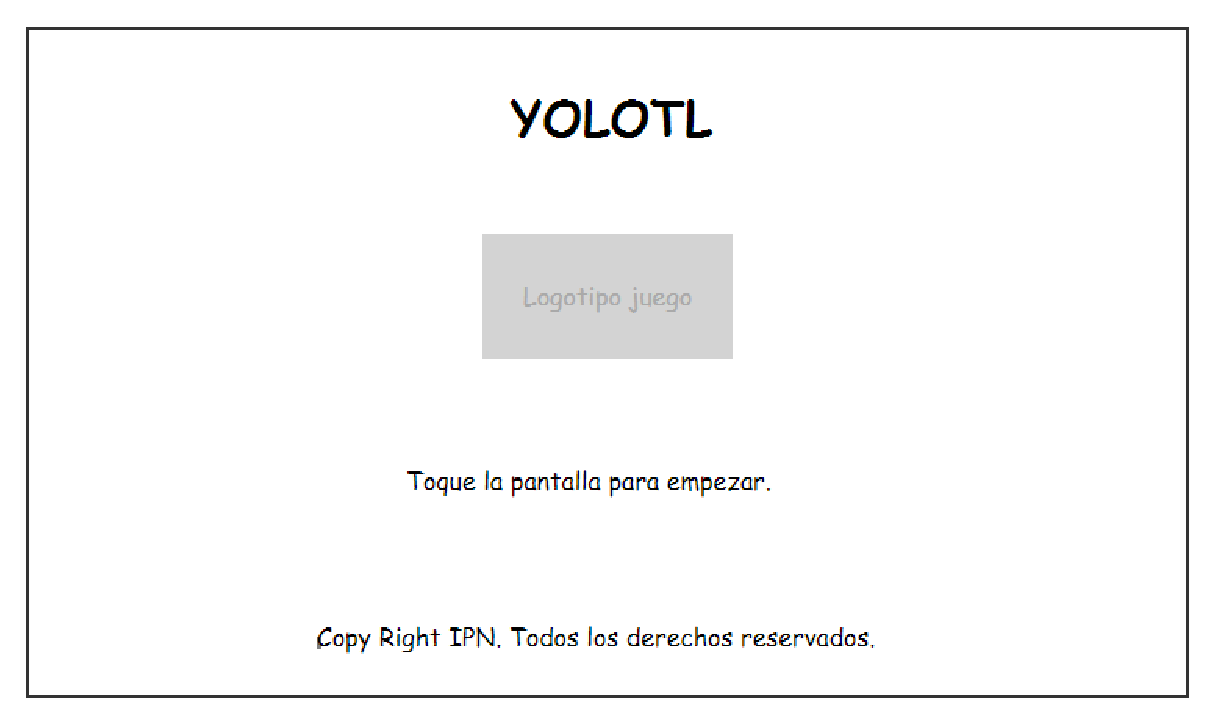
\includegraphics[width=0.6 \textwidth]{05TrabajoRealizado/01DocDiseno02/imagenes/interfaz00}
  \caption{Interfaz 1.0 Pantalla de inicio.}
  \label{fig:PInicio}
\end{figure} 


\begin{figure}
  \centering
   \subfigure[Menú principal] {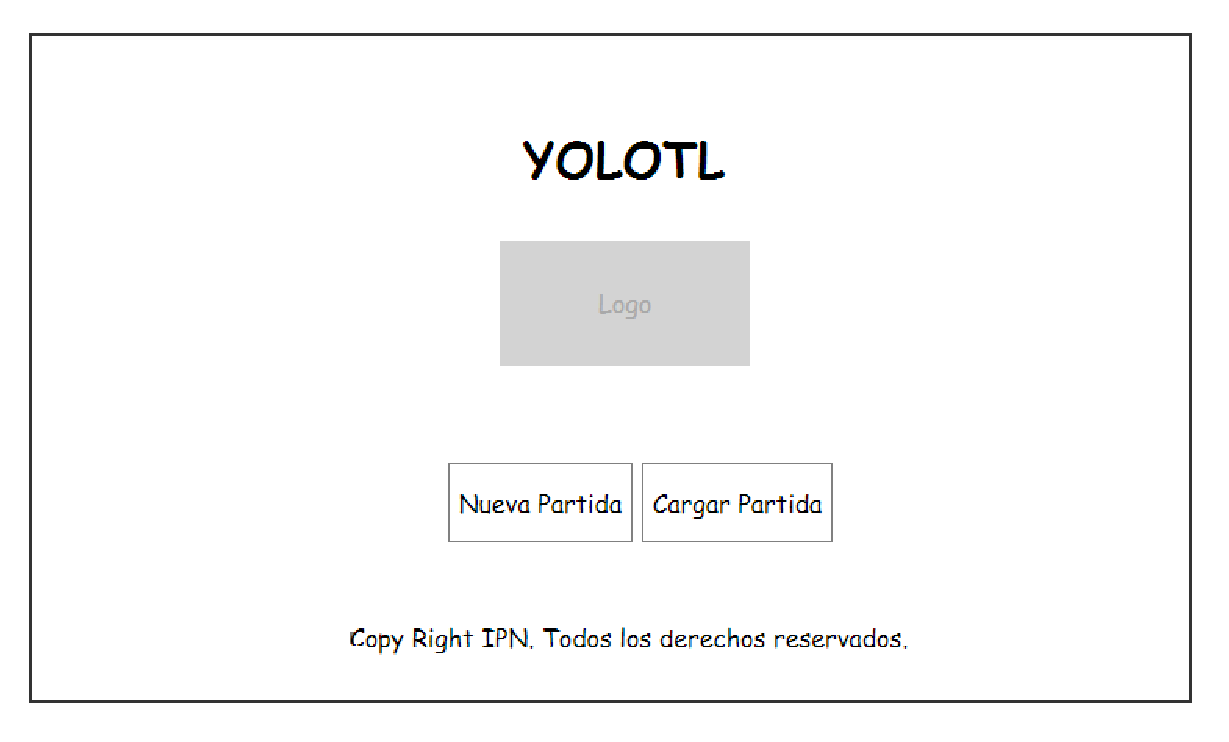
\includegraphics[width=0.6 \textwidth]{05TrabajoRealizado/01DocDiseno02/imagenes/interfaz01}}
   
 	\subfigure[Cuadro de dialogo para confirmar iniciar nueva partida.] {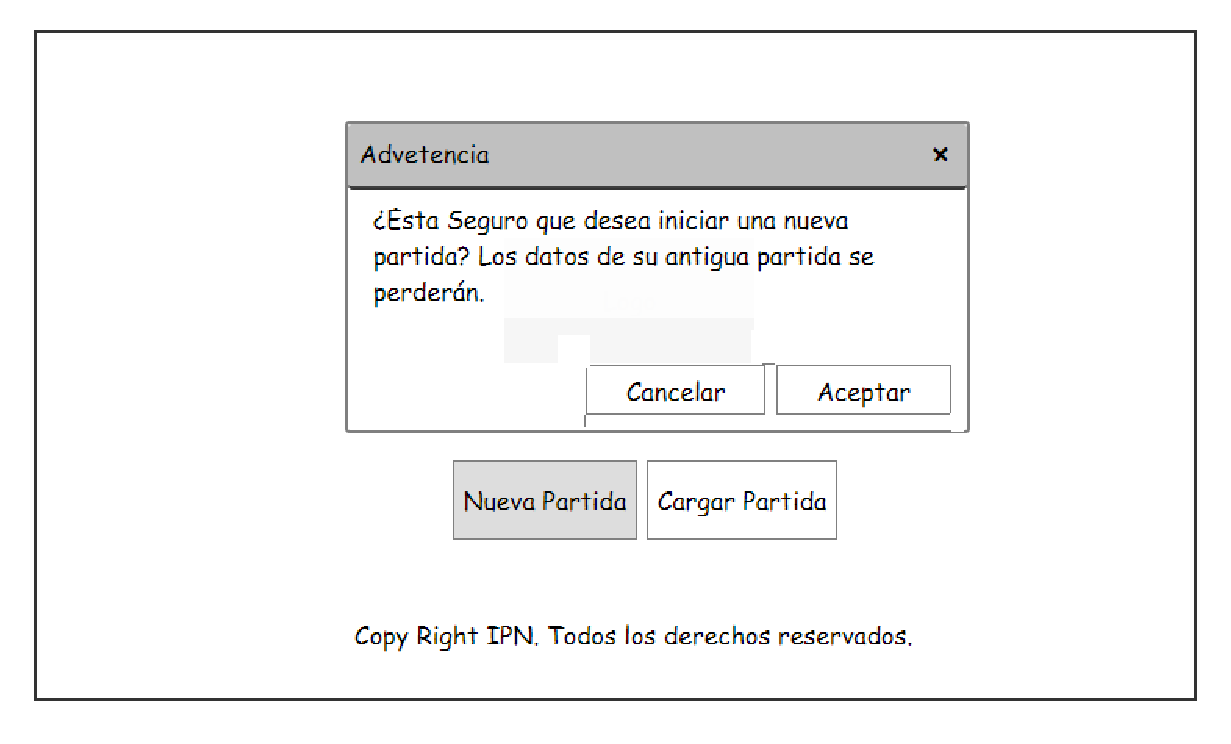
\includegraphics[width=0.6 \textwidth]{05TrabajoRealizado/01DocDiseno02/imagenes/interfaz01_02}}
 	
\subfigure[Cuadro de dialogo cuando no existen partidas que cargar.] {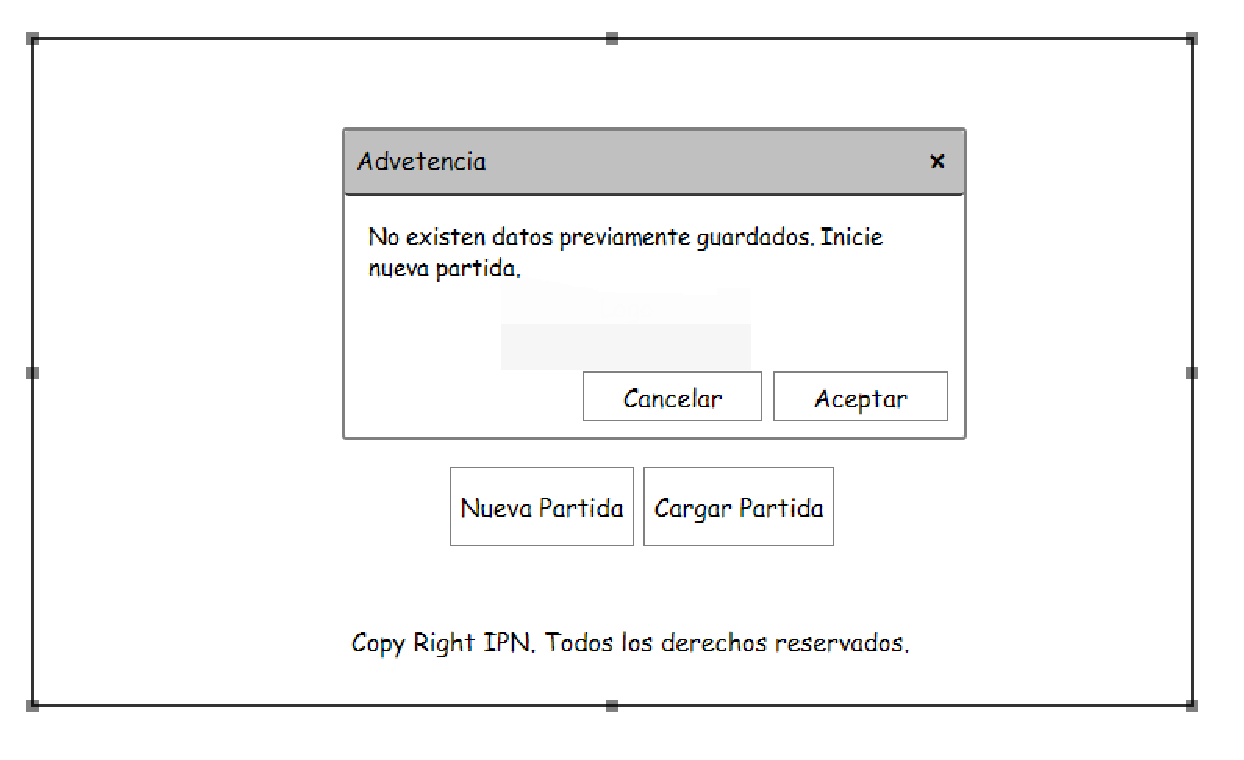
\includegraphics[width=0.6 \textwidth]{05TrabajoRealizado/01DocDiseno02/imagenes/interfaz01_03}}
  \caption{Interfaz 2.00 Menú principal.}
  \label{fig:PMenuP}
\end{figure} 


\begin{figure}
  \centering
   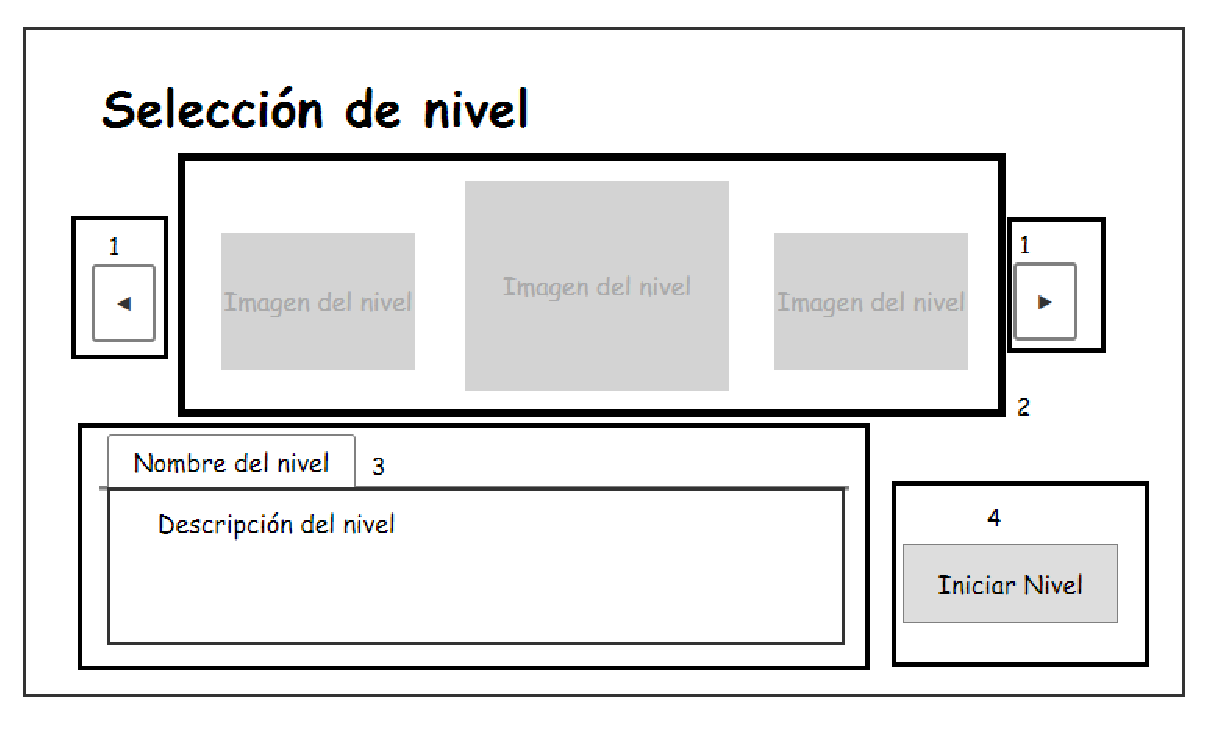
\includegraphics[width=0.6 \textwidth]{05TrabajoRealizado/01DocDiseno02/imagenes/interfaz02_01}
  \caption{Interfaz 2.00 Selección de nivel.1 botones que controlan el carrusel. 2 Carrusel. 3 Información del nivel seleccionado. 4 Botón Iniciar nivel.}
  \label{fig:SelNivel}
\end{figure} 